\documentclass[a4paper,fleqn]{cas-sc}
\usepackage{fontspec}
\usepackage{polyglossia}
\setmainlanguage{vietnamese}
\setotherlanguage{english}
\setmainfont{Times New Roman}
\usepackage{amsmath,amssymb,booktabs,graphicx,hyperref,siunitx,microtype}
\usepackage[numbers]{natbib}
\graphicspath{{../results/analysis_20261018_report/}}
\sisetup{output-decimal-marker={,},group-separator={.}}
\linespread{1.02}
\setlength{\parindent}{1.5em}
\setlength{\parskip}{0pt}
\begin{document}
\title{Mã hóa và thực nghiệm giải bài toán N-Queens bằng SAT, CP và MIP}
\author[1]{Bùi Quang Huy}
\affiliation[1]{organization={UET, K68-CS1},city={Hà Nội},country={Việt Nam}}
\begin{abstract}
Báo cáo nghiên cứu cách giải bài toán N-Queens bằng SAT và đánh giá ba mã hóa ràng buộc at-most-one (AMO): pairwise, sequential và bitwise trên cùng bộ giải Glucose3. Các mô hình đối chiếu gồm OR-Tools CP-SAT, IBM CP Optimizer, IBM CPLEX MIP và Gurobi MIP. Lượt chạy chính thức dùng $N\in\{8,16,32,64\}$, năm phép đo lặp cho mỗi cấu hình, timeout 60 giây và thực thi tuần tự. Nhóm so sánh encoding thu được 60/60 lần SAT hợp lệ. Hai lượt so sánh phương pháp ghi 125 lần SAT hợp lệ và 15 lần UNAVAILABLE do giới hạn license của CPLEX và Gurobi. Kết quả cho thấy kích thước CNF không đủ để dự đoán thời gian giải: pairwise có nhiều clause nhất nhưng ổn định hơn ở các kích thước lớn đã thử. Kết luận chỉ áp dụng cho nhiệm vụ tìm một nghiệm, các kích thước và môi trường đã ghi nhận; nó không chứng minh một encoding hay backend luôn tốt nhất.
\end{abstract}
\begin{keywords}N-Queens \sep SAT \sep AMO \sep CP-SAT \sep MIP \sep Glucose3\end{keywords}
\maketitle

\section{Introduction}
Bài toán N-Queens yêu cầu đặt $N$ hậu trên bàn cờ $N\times N$ sao cho không có hai hậu cùng hàng, cột hoặc đường chéo. Đây là một bài toán thỏa mãn ràng buộc quen thuộc, nhưng vẫn đủ giàu cấu trúc để quan sát sự khác biệt giữa các cách biểu diễn. Trong dự án này, nhiệm vụ được giữ cố định là tìm một nghiệm hợp lệ, không đếm hoặc liệt kê toàn bộ nghiệm.

Ba câu hỏi được đặt ra. Thứ nhất, khi giữ nguyên Glucose3, ba mã hóa AMO ảnh hưởng thế nào đến kích thước CNF và thời gian chạy? Thứ hai, kết quả thay đổi ra sao khi chuyển sang mô hình biến nguyên của CP-SAT hoặc mô hình tuyến tính nguyên của CPLEX? Thứ ba, với các bài toán nhỏ, chi phí dựng mô hình và khởi động tiến trình chiếm tỷ trọng như thế nào so với thời gian giải thực sự?

\section{Background}
SAT tìm một phép gán làm công thức Boolean đúng. Trong dự án, công thức được đưa về dạng chuẩn hội (CNF), tức hội của các mệnh đề tuyển. Với một nhóm biến $S$, ALO là $\bigvee_{x\in S}x$, AMO yêu cầu có nhiều nhất một biến đúng, còn EO là ALO kết hợp AMO. PySAT cung cấp giao diện tạo CNF và gọi solver, đồng thời hỗ trợ các encoding cardinality dùng trong thực nghiệm \cite{pysat,sinz}.

Constraint Programming (CP) mô hình hóa trực tiếp biến miền hữu hạn và ràng buộc toàn cục. Mixed-Integer Programming (MIP) dùng biến nguyên hoặc nhị phân cùng các phương trình, bất phương trình tuyến tính. Ba cách tiếp cận cùng giải N-Queens nhưng không dùng cùng biểu diễn, cơ chế suy diễn hay heuristic; vì vậy phần so sánh backend là so sánh hệ thống hoàn chỉnh, không phải thí nghiệm cô lập một thuật toán lõi.

\section{Methods}
\subsection{Mô hình Boolean}
Biến gốc $x_{r,c}$ có ID $rN+c+1$ và chiếm miền $1,\ldots,N^2$. Mỗi hàng và cột dùng EO. Hai họ đường chéo $r-c$ và $r+c$ dùng AMO, không thêm ALO. Không dùng symmetry breaking.

\subsection{Ba mã hóa AMO}
Pairwise thêm $\binom{k}{2}$ mệnh đề $(\neg x_i\lor\neg x_j)$ cho nhóm $k$ biến và không tạo biến phụ. Sequential dùng bộ đếm tuần tự của PySAT với \texttt{CardEnc.atmost}, \texttt{bound=1} và \texttt{EncType.seqcounter}. Bitwise gán một mã nhị phân cho từng biến gốc; nếu một biến đúng, các bit phụ phải mang mã tương ứng. Hai biến khác nhau không thể cùng đúng vì mã của chúng khác nhau ở ít nhất một bit.

Sequential và bitwise dùng một \texttt{IDPool} chung, bắt đầu sau $N^2$, nên biến phụ không trùng biến bàn cờ hoặc biến phụ của nhóm khác. Tính đúng được kiểm tra theo ngữ nghĩa tồn tại: sau khi cố định phép gán biến gốc bằng assumptions, solver kiểm tra xem có tồn tại cách gán các biến phụ để thỏa CNF hay không.

\subsection{Mô hình đối chiếu}
CP-SAT và CP Optimizer dùng $q_r\in\{0,\ldots,N-1\}$ cùng ba ràng buộc AllDifferent cho $q_r$, $q_r+r$ và $q_r-r$ \cite{ortools,ibmpip}. CPLEX và Gurobi dùng cùng mô hình MIP: biến nhị phân $x_{r,c}$, tổng hàng/cột bằng một và tổng trên mỗi đường chéo không vượt quá một; không có mục tiêu thực chất và dừng sau nghiệm khả thi đầu tiên \cite{ibmlicense,gurobi}. Cách bố trí này giúp hai MIP dùng cùng mô hình toán học, nhưng so sánh SAT, CP và MIP vẫn thay đổi đồng thời cả biểu diễn lẫn backend.

\subsection{Giải mã và xác minh}
SAT chỉ lấy literal dương trong $1\ldots N^2$. Hai backend CP chuyển $q_r$ thành $(r,q_r)$; CPLEX và Gurobi kiểm tra dung sai tích phân trước khi giải mã. Mọi nghiệm đều qua validator độc lập, kiểm tra đủ $N$ tọa độ, hàng/cột và hai họ đường chéo.

\section{Experimental Setup}
Máy chạy Windows 11, Python 3.14.6, 12 logical CPU và khoảng 16 GB RAM. Các phiên bản chính là python-sat 1.9.dev16, Glucose3, OR-Tools 9.15.6755, CPLEX distribution 22.2.0.1, DOcplex 2.32.264 và gurobipy 13.0.3. CPLEX dùng Community Edition; Gurobi dùng restricted non-production license hết hạn ngày 29-11-2027. Thông tin đầy đủ được lưu trong \texttt{environment.json}. Các backend CP/MIP dùng một worker/thread và seed 0; API Glucose3 đang dùng không cho phép điều khiển tương đương.

\texttt{parent\_observed\_time} được đo ở tiến trình cha và bao gồm spawn, import, IPC cùng toàn bộ công việc trong worker. Các trường \texttt{build\_time}, \texttt{load\_time}, \texttt{solve\_time} và \texttt{total\_time} được giữ riêng khi đo được. Năm lần trên cùng $N$ là năm phép đo lặp của một instance chuẩn, không phải năm instance độc lập.

Pilot dùng $N=8,16,32,64$, một lần cho mỗi cấu hình và timeout 10 giây. Lượt chính thức giữ dãy này, chạy năm lần, timeout 60 giây và thực thi tuần tự. Gurobi và CP Optimizer được bổ sung bằng một pilot rồi một run chính thức riêng, cùng dãy $N$ và giao thức. Không chạy $N=128,256$ vì pilot SAT đã có timeout, trong khi CNF pairwise tại $N=64$ đã có 428.864 clause. Dữ liệu thô nằm trong các thư mục run chính thức; bảng và hình được tính từ JSONL/CSV, không sao chép từ README.

\section{Results and Discussion}
\subsection{Trạng thái}
Nhóm A hoàn thành 60/60 lần chạy với trạng thái SAT và tất cả đều có \texttt{validated=true}. Nhóm B ban đầu ghi 100 bản ghi: 90 SAT và 10 UNAVAILABLE; CPLEX bị giới hạn tại $N=32,64$. Run bổ sung ghi 40 bản ghi: 35 SAT và 5 UNAVAILABLE; Gurobi bị giới hạn tại $N=64$, còn CP Optimizer hoàn thành 20/20 lần SAT. Không có TIMEOUT, ERROR hoặc UNKNOWN trong các lượt chính thức. Timeout và unavailable không được đưa vào thống kê thời gian thành công.

\begin{table}[t]\centering
\caption{Tổng hợp trạng thái các lượt chính thức.}\label{tab:status}
\begin{tabular}{lrrrrr}\toprule
Nhóm & SAT & UNSAT & TIMEOUT & ERROR & UNAVAILABLE\\\midrule
Encoding SAT & 60 & 0 & 0 & 0 & 0\\
SAT, CP-SAT, CPLEX & 90 & 0 & 0 & 0 & 10\\
Gurobi, CP Optimizer & 35 & 0 & 0 & 0 & 5\\\bottomrule
\end{tabular}
\end{table}

\subsection{Thời gian}
\begin{table}[t]\centering\caption{Trung vị thời gian cha quan sát (giây), nhóm B; IQR trong ngoặc.}\label{tab:time}
\begin{tabular}{lrrrr}\toprule
Cấu hình & 8 & 16 & 32 & 64\\\midrule
SAT pairwise &0,286 (0,004)&0,308 (0,019)&0,317 (0,006)&0,630 (0,052)\\
SAT sequential&0,284 (0,005)&0,285 (0,006)&0,791 (0,007)&11,339 (0,153)\\
SAT bitwise&0,285 (0,002)&0,408 (0,008)&17,777 (0,225)&7,355 (0,112)\\
CP-SAT&1,077 (0,011)&1,116 (0,032)&1,190 (0,115)&1,436 (0,003)\\
CPLEX MIP&0,478 (0,033)&0,466 (0,018)&--&--\\
Gurobi MIP&0,387 (0,011)&0,380 (0,008)&0,411 (0,011)&--\\
CP Optimizer&1,461 (0,020)&1,486 (0,032)&1,475 (0,020)&1,495 (0,001)\\\bottomrule
\end{tabular}\end{table}
Pairwise là cấu hình ổn định nhất ở $N=16$--$64$ trong dãy đã thử, dù có nhiều clause nhất. Sequential có ít clause hơn nhưng solve tăng mạnh ở $N=64$; bitwise có đỉnh lớn tại $N=32$. Đây là mô tả có điều kiện, không phải định luật đơn điệu hay kết luận phổ quát.

\begin{table}[t]\centering\caption{Kích thước CNF tại $N=64$.}\label{tab:size}
\begin{tabular}{lrrrr}\toprule Encoding & Biến bàn cờ & Biến phụ & Tổng biến & Clause\\\midrule
Pairwise&4096&0&4096&428864\\
Sequential&4096&15998&20094&47752\\
Bitwise&4096&2036&6132&95572\\\bottomrule
\end{tabular}\end{table}
Ít clause không đảm bảo nhanh hơn: số biến phụ, cấu trúc mệnh đề, propagation, heuristic và overhead đều ảnh hưởng. Với $N=8$, solve của các backend native rất nhỏ nhưng thời gian cha quan sát lớn hơn nhiều, cho thấy chi phí khởi động/import quan trọng. Trường \texttt{load\_time=null} của CP/MIP có nghĩa là không đo tách được, không phải bằng không. Số liệu Gurobi chỉ đến $N=32$ và số liệu CPLEX chỉ đến $N=16$, nên không dùng các trung vị còn lại để suy luận cho kích thước lớn hơn.

\begin{figure}[t]\centering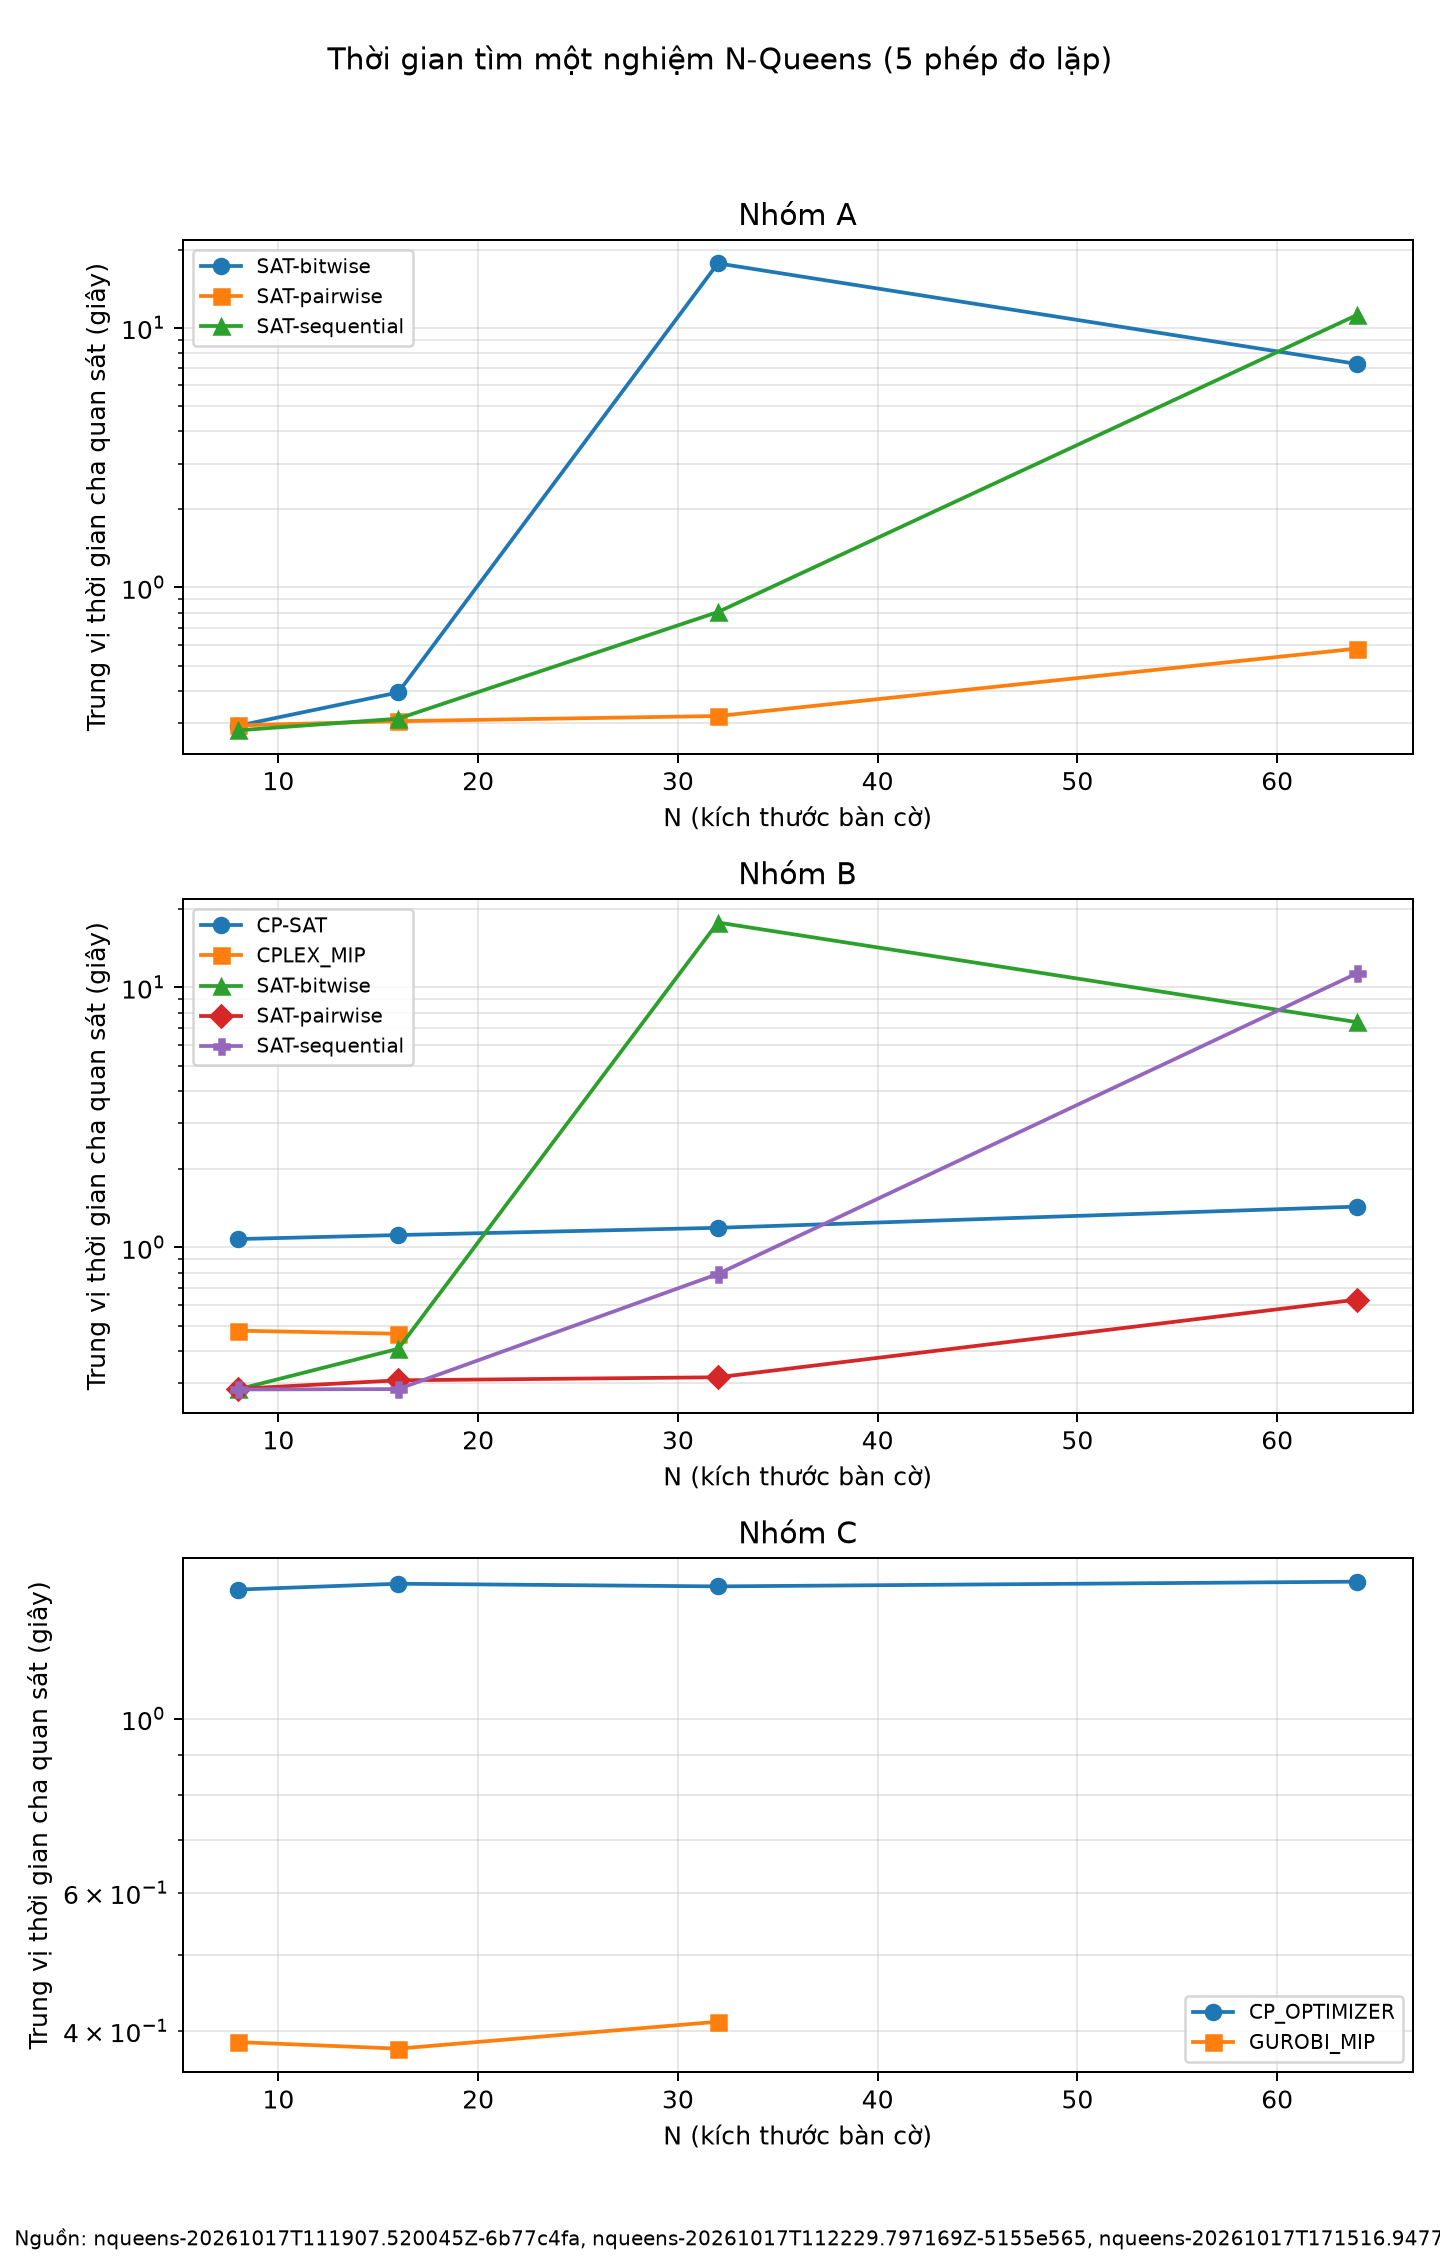
\includegraphics[width=0.95\linewidth]{time_by_n.png}\caption{Thời gian theo $N$; timeout được xử lý riêng trong script. Nguồn: \texttt{results/analysis\_20261018\_report/summary.csv}.}\label{fig:time}\end{figure}
\begin{figure}[t]\centering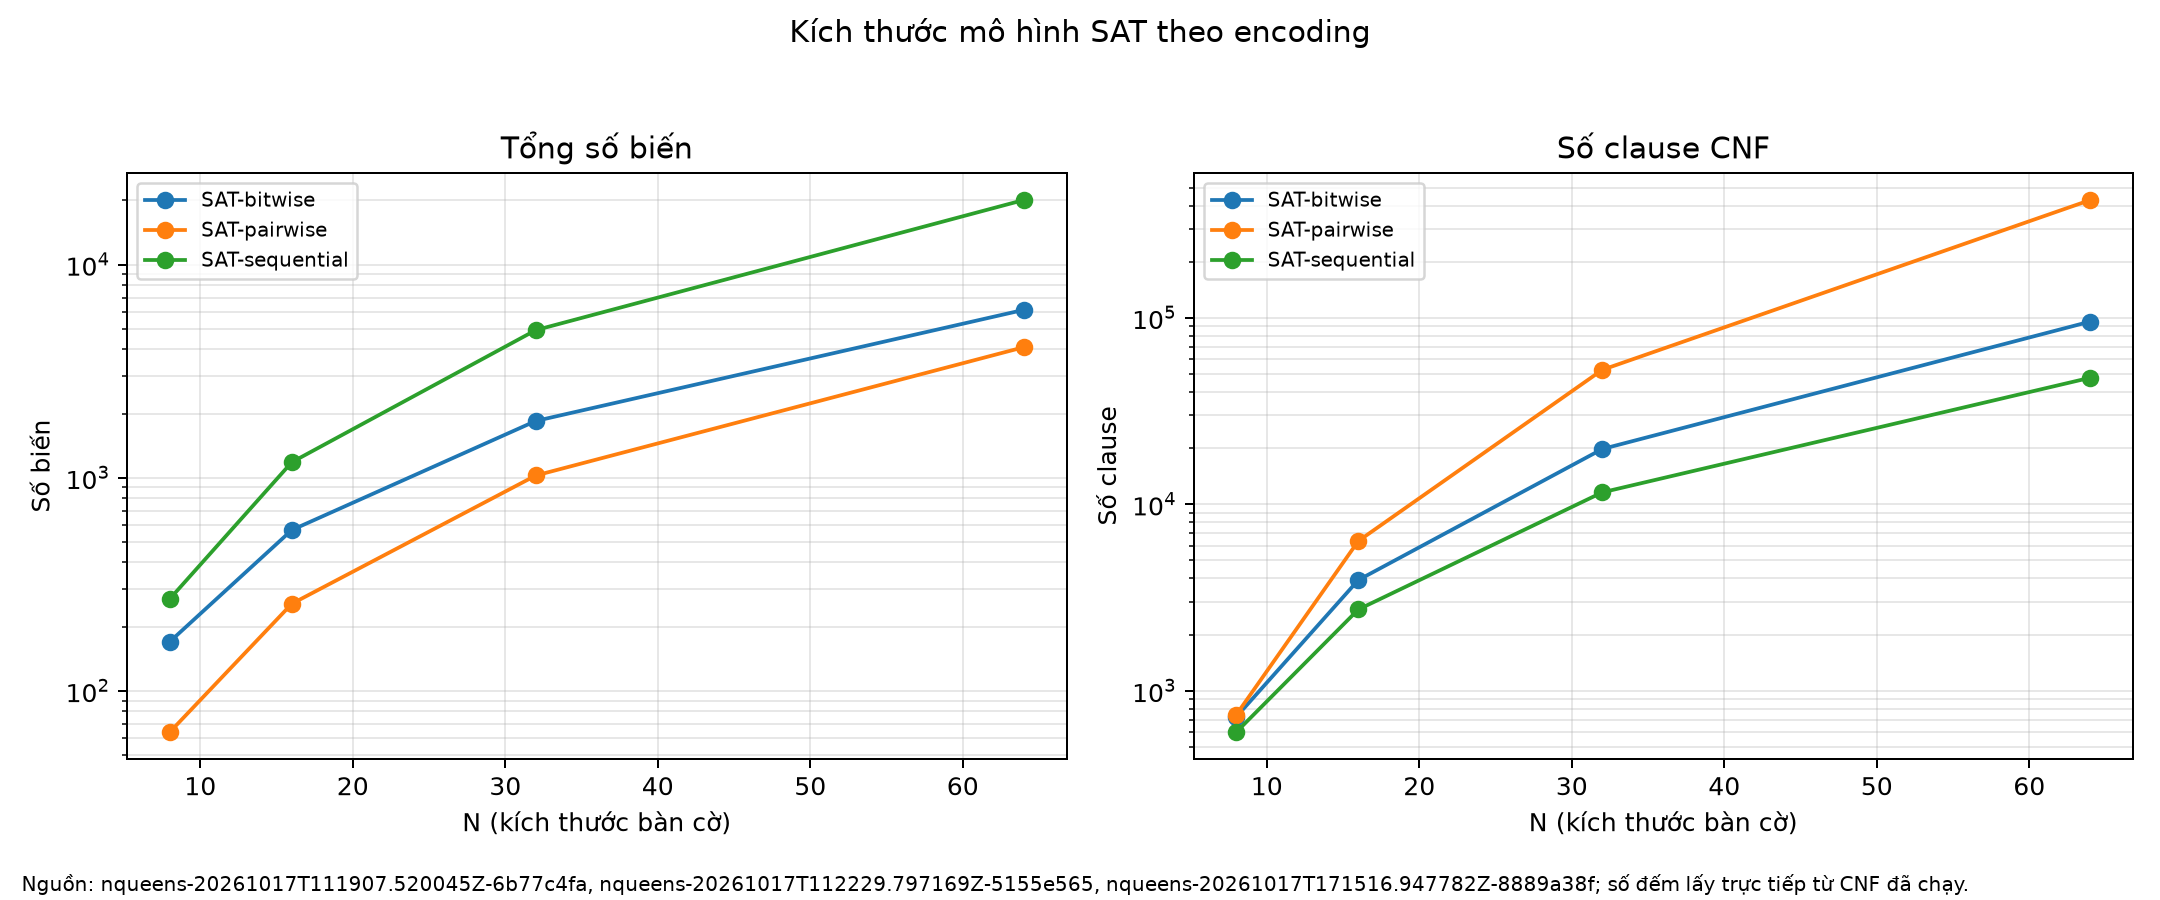
\includegraphics[width=0.95\linewidth]{sat_model_size.png}\caption{Số biến và clause của các encoding SAT. Nguồn: \texttt{results/analysis\_20261018\_report/summary.csv}.}\label{fig:size}\end{figure}
\begin{figure}[t]\centering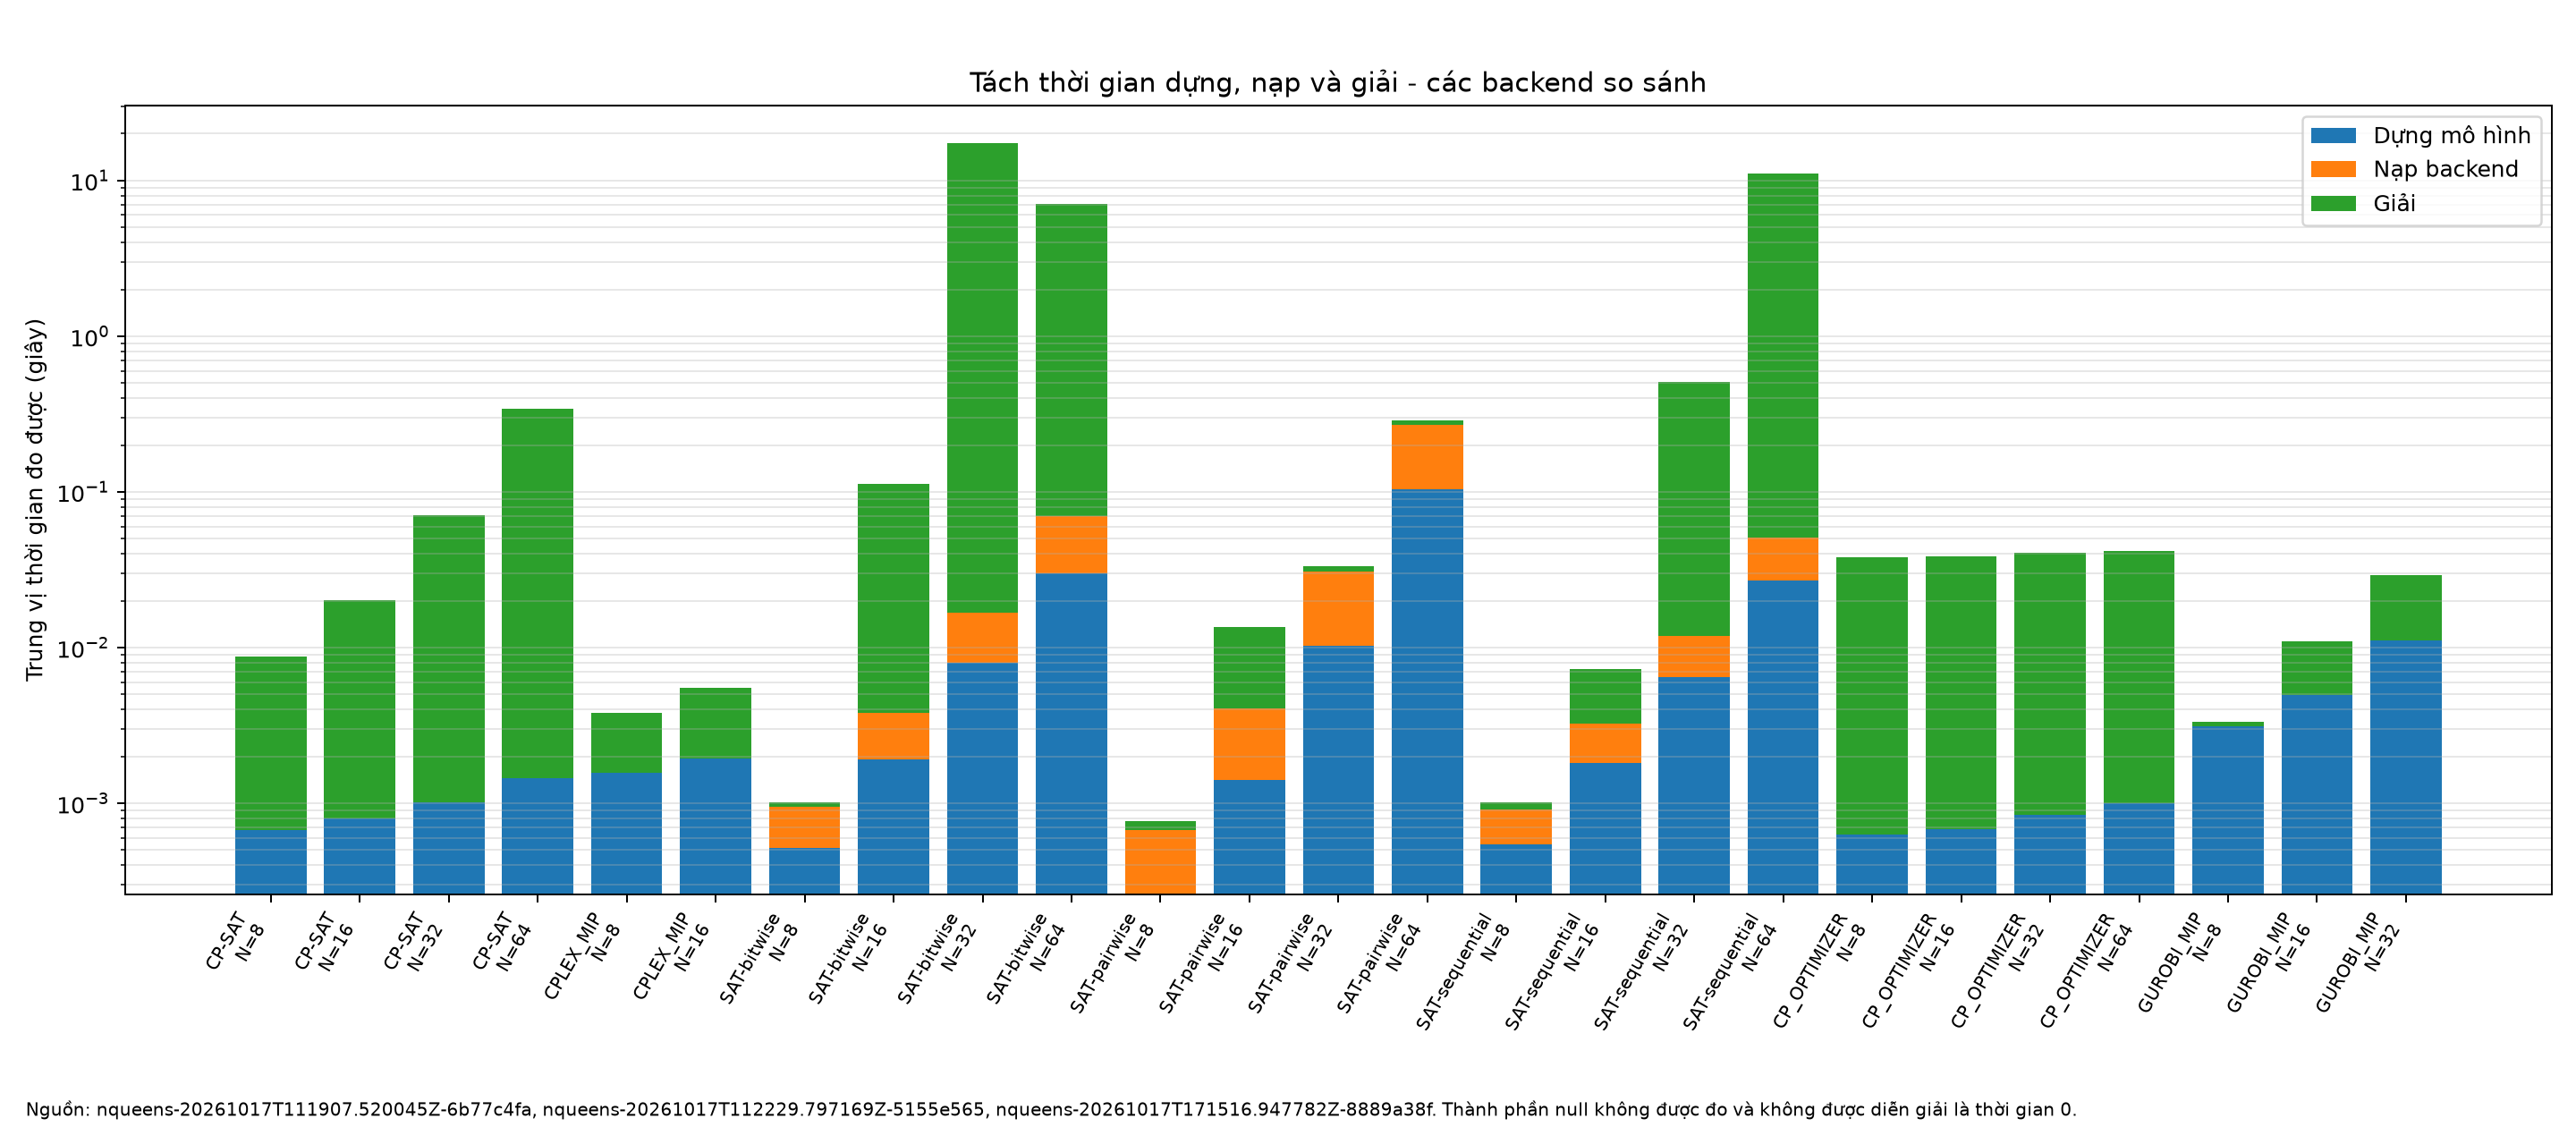
\includegraphics[width=0.95\linewidth]{phase_times.png}\caption{Các pha build, load và solve khi dữ liệu đo được; giá trị null không được diễn giải là số đo bằng không.}\label{fig:phase}\end{figure}

\subsection{Giới hạn của thực nghiệm}
Thực nghiệm chỉ xét bốn kích thước và một instance N-Queens chuẩn tại mỗi kích thước. Các lần lặp giúp mô tả độ dao động thời gian nhưng không tạo thêm tính đa dạng cho tập bài toán. $N=64$ là kích thước lớn nhất được chọn sau pilot; $N=128,256$ chưa chạy vì pilot đã cho thấy timeout ở một số encoding và pairwise tăng nhanh về số clause. Kết quả còn phụ thuộc máy, phiên bản Python, phiên bản solver, license và cơ chế khởi động tiến trình trên Windows. Ngoài ra, SAT, CP-SAT và MIP thay đổi đồng thời mô hình lẫn backend, nên chênh lệch quan sát được không thể quy hoàn toàn cho một thuật toán giải.

\section{Conclusion}
Dự án đã hoàn thành pipeline SAT ba encoding, CP-SAT, CP Optimizer, CPLEX MIP và Gurobi MIP trong môi trường hiện có. Pairwise cho thời gian thấp và ổn định nhất ở các kích thước lớn đã thử, nhưng bằng chứng chỉ gồm bốn $N$ và một instance mỗi $N$. CPLEX chỉ có dữ liệu $N=8,16$; Gurobi chỉ có dữ liệu đến $N=32$ vì giới hạn license. Không thể kết luận backend hay encoding nào luôn tốt nhất, cũng không thể suy rộng sang đếm hoặc liệt kê nghiệm.

\section{Data Availability}
Mã nguồn, cấu hình thực nghiệm, JSONL thô, CSV, script phân tích và các hình được công bố tại \url{https://github.com/pr0f1Ne/nqueens-sat}. Có thể tái tạo tổng hợp bằng:
\begin{verbatim}
.venv\Scripts\python.exe analyze_results.py --group-a results\official_group_a\nqueens-20261017T111907.520045Z-6b77c4fa --group-b results\official_group_b\nqueens-20261017T112229.797169Z-5155e565 --group-c results\official_commercial_completion\nqueens-20261017T171516.947782Z-8889a38f --output results\analysis_reproduced
\end{verbatim}
Run bổ sung Gurobi/CP Optimizer nằm tại \texttt{results/official\_commercial\_completion/nqueens-20261017T171516.947782Z-8889a38f/}.

\section*{References}
\begin{thebibliography}{9}
\bibitem{pysat} A. Ignatiev, A. Morgado, J. Marques-Silva, ``PySAT: A Python toolkit for prototyping with SAT oracles,'' in \textit{SAT 2018}, pp. 428--437, 2018. doi: \url{https://doi.org/10.1007/978-3-319-94144-8_26}.
\bibitem{sinz} C. Sinz, ``Towards an optimal CNF encoding of Boolean cardinality constraints,'' in \textit{CP 2005}, pp. 827--831, 2005. doi: \url{https://doi.org/10.1007/11564751_73}.
\bibitem{ortools} Google OR-Tools, ``CP-SAT solver,'' \url{https://developers.google.com/optimization/cp/cp_solver}.
\bibitem{ibmpip} IBM, ``CPLEX Python API now installed using pip/conda,'' \url{https://www.ibm.com/docs/en/icos/22.1.2?topic=rnco2-cplex-python-api-now-installed-using-pip-conda}.
\bibitem{ibmlicense} IBM, ``CPLEX Optimization Studio pricing and editions,'' \url{https://www.ibm.com/products/ilog-cplex-optimization-studio/pricing}.
\bibitem{gurobi} Gurobi Optimization, LLC, ``Gurobi Optimizer Python API,'' \url{https://docs.gurobi.com/projects/optimizer/en/current/reference/python.html}.
\bibitem{project} B. Q. Huy, ``N-Queens SAT project,'' mã nguồn và dữ liệu thực nghiệm, \url{https://github.com/pr0f1Ne/nqueens-sat}.
\end{thebibliography}
\end{document}
